\chapter{Realisieren}\label{ch:realisieren}
In diesem Kapitel wird die IPERKA-Phase Realisieren dokumentiert. Es werden die Wichtigsten und entscheidenen Punkte während der Implentierung festgehalten. 

\section{Backend erweitern}
In diesem Abschnitt wird die Implementierung des Backends dokumentiert. 
\subsection{Neuer REST-Endpunkt}
Als ersten Schritt wurde der neue REST-Endpunkt erstellt:
\begin{lstlisting}[language=Java]
	@JsonApiResource(attributes = Airlock2FAShortActivationCodeData.class)
@Path("activation-code-short")
public Response getShortActivationCode (@ExistingUser @PathParam("userId") @Parameter(schema = @Schema(type = "string")) UserParam userParam) {
	return ok(new Airlock2FAShortActivationCodeData(null)).build();
}
\end{lstlisting}
Der Endpunkt sieht aktuell so aus. Es sind noch keinerlei Funktionalitäten implementiert. Daher wird auch hardcoded null zurückgegeben. Airlock2FAShortActivationCodeData.java ist das Dataobjekt welches ein nullable Feld \flqq short\_activation\_code\frqq{} enthält. \\
\\
\textbf{Rolebased Access Control}\\
Damit der Zugriff auf den neuen Endpunkt nur dann funktioniert, wenn der Admin die nötigen Rollen dazu besitzt, musste eine neue RestAction definiert werden. Diese wird in der Klasse RestActionsDefinitions.java folgendermassen erstellt:
\begin{lstlisting}[language=Java]
	public static RestAction viewAirlock2FAActivationCode () {
	return RestAction
	.builder()
	.action(viewAirlock2FAActivationSecret)
	.rule(Rule.of(GET, "/users/[^/]+/tokens/airlock-2fa/activation-code-short"))
	.build();
}
\end{lstlisting}
Dies bewirkt nun, dass die Action \flqq viewAirlock2FASecrets\frqq{}, welche es schon gab, auf diesen Pfad matched. Das heisst bei jedem Call auf den neuen Endpunkt, wird zuerst validiert, ob der Nutzer die richtigen Rollen hat, welche für diese Action benötigt werden, ansonsten wird 403 zurückgegen.
Ein Problem hat sich nun hervorgehoben. Es gibt bereits folgendes Pattern:\\
 \flqq .rule(Rule.of(GET, "\verb*|text/users/[^/]+/tokens/airlock-2fa(/.*)?"))|\frqq{}
\\
Dieses Pattern matched auch auf den neuen Pfad. Da dieses Pattern in der allgemeine Action \flqq viewToken \frqq{} definiert wurde, könnte es nun zu Konflikten kommen. Deshalb wurde der neue Pfad in diesem Pattern mit Hilfe eines Negative Lookaheads ausgeklammert. Das neue Pattern für die viewToken Action sieht nun so aus:\\


\noindent \verb @/users/[^/]+/tokens/airlock-2fa(?!/activation-code-short(?:/|$))(/.*)?\$ @\\\\
So kann die viewAirlock2FAActivationSecrets Action unabhängig von der viewToken Action konfiguriert werden. Es entstehen dementsprechend keine fehlkonfigurationen und überschreibungen der Mappings.\\
\\
\textbf{REST-Dokumentation}\\
Eine Anforderung an neue REST-Endpunkte ist deren Dokumentation. Zum Zeitpunkt der Probe-IPA wird diese mit Miredot via Javadoc generiert. Sprich Miredot erstellt eine REST-Dokumentation, basiernd auf dem Javadoc. Für den neuen Endpunkt setzt sich diese Dokumentation wie folgt zusammen:
\begin{figure}[H]
	\begin{center}
		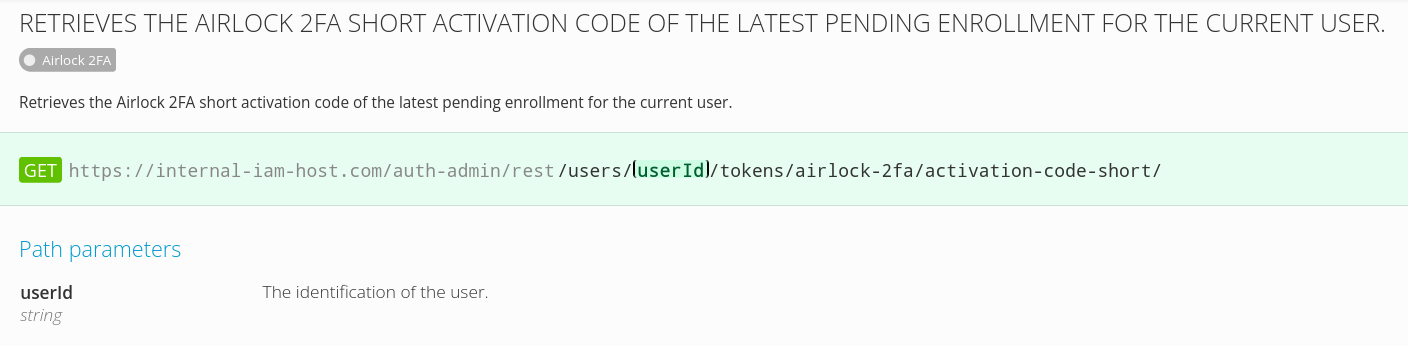
\includegraphics[width=1.0\textwidth]{ressourcen/requestdoc}
		\caption[REST-Dokumentation Request]{Miredot REST-Dokumentation Request}\label{fig:requestdoc}
	\end{center}
\end{figure}
\noindent Zu oberst ist immer der Titel des Requests. Darunter folgt eine Kurze Zusammenfassung. Danach ist der Pfad dargestellt mit der entsprechenden HTTP-Methode.
Zum Schluss folgen die Pfadparamter, was in diesem Fall die User ID ist.
Anschliessend folgt die Response:

\begin{figure}[H]
	\begin{center}
		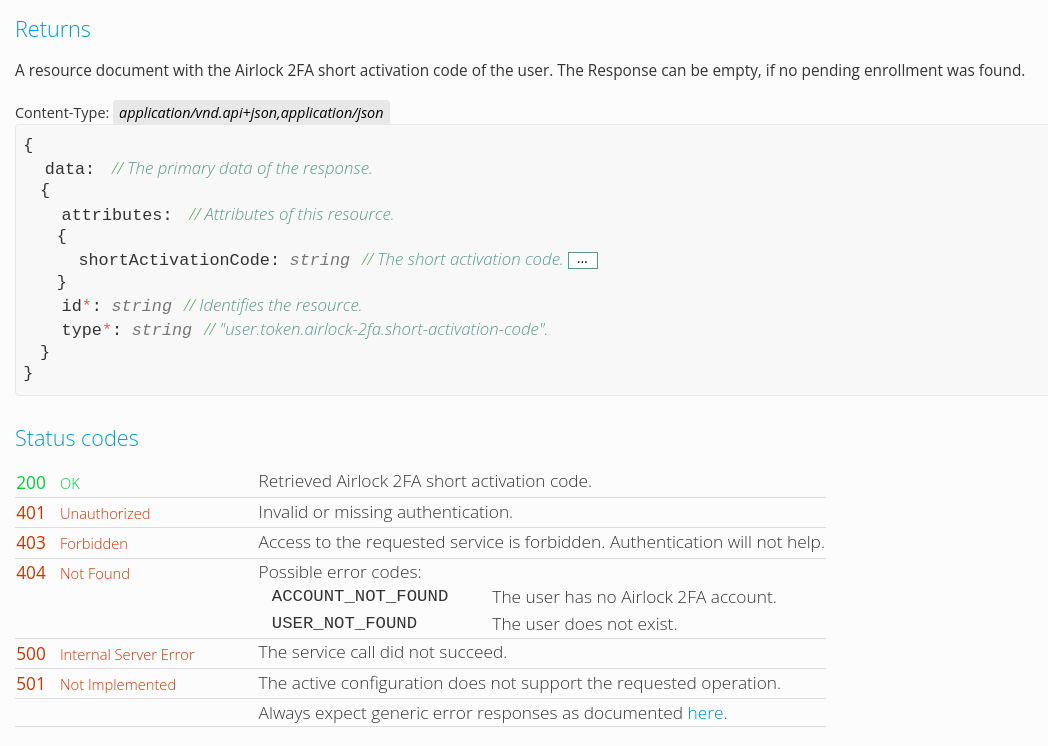
\includegraphics[width=1.0\textwidth]{ressourcen/responsedoc}
		\caption[REST-Dokumentation Response]{Miredot REST-Dokumentation Response}\label{fig:responsedoc}
	\end{center}
\end{figure}

\subsection{Requests zu Futurae}
Damit die SPA den 16-stelligen Aktivierungscode wie geplant angeboten bekommt, müssen in der Kommunikation zwischen IAM und Futurae einige Erweiterungen getroffen werden.\\
\\
\textbf{16-stelliger Aktivierungscode erzwingen}\\
Damit der 16-stellige Aktivierungscode bei dem Request, welcher das neuste offene Enrollment sucht, auch zurück kommt musste zuerst sichergestelt werden, dass bei dem Enrollment Request das Property \flqq shortcode\frqq{} auf true gesetzt wird. Dafür wurde auf dem Request Objekt ein weiteres Feld hinzugefügt.\\
Hier galt es zu beachten, dass jeweils 2 verschiedene Enrollment Requests gemacht werden:
\begin{itemize}
	\item Für einen neuen Nutzer, sprich ohne Account.
	\item Für einen Nutzer welcher schon einen Account besitzt. 
\end{itemize}
Dies musste sowohl für den Adminapp API Call zu Futurae als auch den Loginapp Call gemacht werden.
\\
\\
Nebst dem Request musste natürlich auch die Response geändert werden, und um dieses Feld erweitert werden.
\\
Zum serealisieren und deserealisieren des Requests- / Response-Body wird Jackson verwendet. Dabei werden mit einfachen Annotationen die Javaobjekte auf die verlangten JSON-Felder gemapped oder umgekehrt:
\captionsetup[lstlisting]{labelformat=empty}
\begin{lstlisting}[language=Java, caption={Beispiel, wie Jackson auf dem Futurae Request zur Auth API (verwendet für die Self-Services) verwendet wird. (Enthält bereits das neue Feld \flqq short\_code\frqq).}]
@NoArgsConstructor
@Getter
@Setter
@JsonInclude(Include.NON_NULL)
public class FuturaeAuthApiEnrollmentRequest {
	
	@JsonProperty("user_id")
	private String userId;
	
	@JsonProperty("username")
	private String username;
	
	@JsonProperty("display_name")
	private String displayName;
	
	@JsonProperty("valid_secs")
	private Integer validSecs;
	
	@JsonProperty("short_code")
	private Boolean shortCode;
	
	@JsonProperty("success_callback_url")
	private String successCallbackUrl;
	
	@JsonProperty("phone_number")
	private String phoneNumber;
	
	@JsonProperty("enrollment_flow_binding_enabled")
	private Boolean enrollmentFlowBindingEnabled;
	
	@JsonProperty("account_recovery_flow_binding_enabled")
	private Boolean recoveryFlowBindingEnabled;
}
\end{lstlisting}
\textbf{Erweitern der Requestfactory}\\
Als nächsten Schritt wurde die FuturaeAdminApiEnrollmentRequestFactory.java um eine neue Methode erweitert:
\begin{lstlisting}[language=Java]
public RestRequest getLatestPendigEnrollment (String airlock2FAAccountId) {
	return futuraeRequestFactory.createGetRequest(ENROLLMENTS.usersPath(), getQueryParams(airlock2FAAccountId));
}

private static Map<String, Object> getQueryParams (String airlock2FAAccountId) {
	return Map.of("user_id", airlock2FAAccountId,
	"status", "pending",
	"sort_by", "created_at",
	"order", "desc",
	"limit", "1");
}
\end{lstlisting}
Diese Methode \flqq getLatestPendingEnrollment\frqq mit der statischen Hilfsmethode \flqq getQueryParams \frqq baut einen GET Request mit folgendem Pfad zusammen:\\\\
/srv/admin/v1/enrollments?user\_id={userid}
\newline\&status=pending 
\newline\&sort\_by=created\_at 
\newline\&order=desc
\newline\&limit=1\\\\
Dies ist der Request, welcher ausgeführt werden muss, um das neuste offene Enrollment zu bekommen.\\\\
\textbf{Erweitern des Enrollment Service}\\
Damit die Response von Futurae richtig geparst werden kann, musste zuerst ein äquivalentes Java Entity Objekt erstellt werden:
\begin{lstlisting}[language=Java]
@Data
@NoArgsConstructor
@AllArgsConstructor
@JsonIgnoreProperties(ignoreUnknown = true)
public class FuturaeAdminEnrollmentListResponse {
	
	@NotNull
	@JsonProperty("count")
	private Integer count;
	@NotNull
	@JsonProperty("enrollments")
	private List<FuturaeAdminEnrollmentResponse> enrollmentResponseList;
	@NotNull
	@JsonProperty("limit")
	private Integer limit;
	@NotNull
	@JsonProperty("offset")
	private Integer offset;
	@NotNull
	@JsonProperty("total")
	private Integer total;
}
\end{lstlisting}
Dieses Objekt bildet folgende JSON-Response, welche von Futurae so definiert wurde,in Java ab:
\begin{verbatim}
{
	"count": 0,
	"enrollments": [{FuturaeAdminEnrollmentResponse}],
	"limit": 0,
	"offset": 0,
	"total": 0
}
\end{verbatim}
Der FuturaeAdminApiEnrollmentServiceImpl.java ist die Schnittstelle zwischen IAM und Futurae, für alle Aktionen welche das Enrollment betreffen. Für das wurde im seinem Interface die Methode \flqq getLatestPendingEnrollment\frqq definiert. Die Implentation sieht folgendermassen aus:
\begin{lstlisting}[language=Java]
@Override
public Optional<Airlock2FAEnrollment> getLatestPendingEnrollment (Airlock2FAAccountId accountId) {
	RestRequest request = 
	adminApiRequestFactory
	.getLatestPendigEnrollment(accountId.getId());
...
\end{lstlisting}
Zuerst wird der Request über die vorhin erstellte Methode zusammengestellt.
Danach wird er via den Restclient ausgeführt. Die Response wird anschliessend im folgenden Responsehandler behandelt:
\begin{lstlisting}[language=Java]
...
return restClient.read(request, response -> {
	if (response.getStatusInfo().equals(BAD_REQUEST)) {
		LOG.info("Invalid parameters for request to fecht latest pending enrollment for account with id: " + accountId.getId());
		return Optional.empty();
	}
	if (!response.getStatusInfo().equals(OK)) {
		LOG.info("Request to fetch the latest pending enrollment for account with id '" + accountId.getId() + "' failed with code: " + response.getStatusInfo());
		return Optional.empty();
	}
	FuturaeAdminEnrollmentListResponse result = readResponse(response, FuturaeAdminEnrollmentListResponse.class, request)
	.orElseThrow(Airlock2FAAdminApiException::new);
	if (result.getEnrollmentResponseList().isEmpty()) {
		LOG.info("Could not find a pending enrollment for account with id: " + accountId.getId());
		return Optional.empty();
	}
	return Optional.of(mapEnrollment(result
	.getEnrollmentResponseList().getFirst()));
});
\end{lstlisting}
Falls die Response einen 400 beinhaltet wird eine Info geloggt und Optional.empty zurück gegben. Dieser Fall sollte eigentlich nicht auftreten es sei denn, die Futurae API ändert sich. Denn dieser Fehler kommt nur dann, wenn die Parameter falsch sind, und diese sind Hardcoded, können also nicht vom Nutzer beeinflusst werden. Um unerwarete Fehler zu vermeiden wird dieser Fall hier dennoch explizit abgefangen.\\
Da dies der einzige von Futurae definierte Error für diesen Request ist, werden die anderen mit dem darauf folgenden if-Statement abgefangen.\\
Danach wird in einem bereits bestehenden ResponseReader die Response in das Erwartete Objekt geparst. Ist das zurückkommende Result präsent, wird geprüft, ob es Einträge in der Enrollmentliste gibt, falls ja wird ein Optional vom ersten Eintrag genommen. Dies geht, da davon ausgegangen werden kann, dass entweder genau 0 oder 1 Eintrag vorhanden ist. Dies weil im Request die limit auf 1 gesetzt wurde.\\
\\
Dieses Optional wird dann über den Airlock2FAAdminService.java an die Resource überliefert, welche dann schlussendlich den Code oder null, falls nichts vorhanden, zurückgibt.
\subsection{Logging}
Das Logging muss die Anforderung \flqq FA 3\frqq , definiert in Abschnitt \ref{subsec:anforderungenBackend} erfüllen. Hierfür wurde im Airlock2FAAdminService.java folgende Methode imlementiert:
\begin{lstlisting}[language=Java]
public Optional<String> findLatestPendingEnrollment (Airlock2FAUserAccount account) {
	return adminApiEnrollmentService
	.getLatestPendingEnrollment(account.getAccountId())
	.map(enrollment -> {
		helpdeskLogger.log(account.getUserId(), format("Administrator '%s' accessed the Airlock 2FA short activation code.", administrator.getName()));
		return enrollment.getActivationCodeShort();
	})
	.or(() -> {
		helpdeskLogger.log(account.getUserId(), format("Administrator '%s' tried to access the Airlock 2FA short activation code but no value was present.", administrator.getName()));
		return Optional.empty();
	});
\end{lstlisting}
In dieser Methode wrid aus dem erhaltenen Optional Enrollment der 16-stellige Aktivierungscode herausgefiltert und je nache fall, ob präsent oder nicht, wird ein Optional String oder Empty zurückgegeben. Da dies der Service ist, welcher der Resource dient, in welcher der neue Endpunkt ist, wurde hier dann das Logging eingebaut. Das heisst diese Methode ist weniger allgemein, als jene im Enrollmentservice und es kann davon ausgegangen werden, dass sie nicht von anderen Features genutzt wird. Da es im User Activities Logfile stehen muss, wurde der Helpdesklogger verwendet. In der Adminapp im Activities Tab des aktuellen Nutzers, sieht dies nun wie folgt aus:
\begin{figure}[H]
	\begin{center}
		
\includegraphics[width=1.0\textwidth]{ressourcen/logpresent}
		\caption[Logeintrag bei vorhandenem Aktivierungscode]{Logeintrag bei vorhandenem Aktivierungscode}\label{fig:logpresent}
	\end{center}
\end{figure}
\noindent Im obigen Bild links, ist der Zeitpunkt, zudem der Admin auf den Code zugegriffen hat, zusehen. Auf der rechten Seite dann der Text, welcher im obigen Code im ersten Logstatement steht. 
\begin{figure}[H]
	\begin{center}
		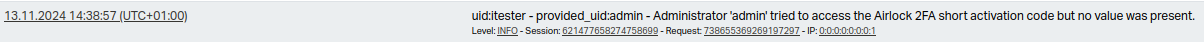
\includegraphics[width=1.0\textwidth]{ressourcen/lognotpresent}
		\caption[Logeintrag bei \textbf{nicht} vorhandenem Aktivierungscode]{Logeintrag bei \textbf{nicht} vorhandenem Aktivierungscode}\label{fig:lognotpresent}
	\end{center}
\end{figure}
\noindent Im obigen Bild links, ist der Zeitpunkt, zudem der Admin auf den Code zugegriffen hat, zusehen. Auf der rechten Seite dann der Text, welcher im obigen Code im zweiten Logstatement steht.  

\subsection{Resultat}
Die oben aufgezeigten Schritte führten schlussendlich zum gewollten Resulat. Der Endpunkt liefert nun den neusten, offenen Aktivierungscode, falls er vorhanden ist
\begin{verbatim}
{
	"shortActivationCode": "60b9 7irw xad1 2w8v"
}
\end{verbatim}
und sonst null resp. nichts.
\begin{verbatim}
	{
		{}
	}
\end{verbatim}
Der Endpunkt ist durch den Role Based Access Controller geschützt, sodass nur Admins mit den nötigen Rollen Zugriff haben. Alle anderen erhalten einen 403. Jeder erlaubte Zugriff wird nach den Anforderungen geloggt.
\subsection{Tests}
















